\section{Background and Related Works}\label{sec:background}
\subsection{Mobile Robot Graph-Based World Models}\label{sec:background_graph_configurations}
In this section we first briefly summarize the use of factor graphs, scene graphs and hybrid forms of both for robotic world modeling. We then define \textit{dynamics} in the context of robotics and finally provide an overview of existing surveys and reviews of the use of factor and scene graphs, particularly for modeling \textit{dynamic} robot environments, and identify research gaps herein, which motivate this review article. 

\subsubsection{Factor Graphs}\label{sec:background_factor_graphs}
Factor graphs have emerged as a primary mathematical framework mainly for geometric world models, providing a flexible approach for integrating various sensor data and prior knowledge into a unified, probabilistic optimization problem\cite{deeb_model-based_2019} \cite{gulati_robust_2017}. In general, a factor graph describes the structure of a factorization of a function. For instance, 
consider a function $J(X)$ of a set of variables $X = \{x_1, \ldots , x_n\}$, that factors into a product of $r$ local functions or ``factors'' $\phi_j(X_j)$ of a subset $X_j$ of $X$, respectively:
\begin{equation}
J(X) = \prod_{j=1}^{r} \phi_j(X_j)
\end{equation}
A factor graph $G = \{X,\mathcal{F},\mathcal{E}\}$ is an undirected bipartite graph that consists of  the set of variable nodes $X$, typically depicted as circles, and the set of factor nodes $\mathcal{F}$, typically depicted as squares. The set $\mathcal{E}$ involves the edges connecting variable nodes and factor nodes. The example in Figure \ref{fig:FG_example} shows a factor graph with
5 variables $X = \{x_1, \ldots, x_5 \}$ and 8 factors $\mathcal{F}=\{\phi_1, \ldots, \phi_8 \}$,  representing the factorization 
\begin{equation}
\begin{aligned}
    J(X) &= \prod_{j=1}^{8} \phi_j(X_j) \\
    &= \phi_1(x_1)\cdot\phi_2(x_1,x_2) \cdot \phi_3(x_2,x_3) \cdot \\
    & \quad \phi_4(x_1,x_4) \cdot \phi_5(x_2,x_4) \cdot \phi_6(x_3,x_5) \cdot \\
    & \quad \phi_7(x_4) \cdot \phi_8(x_5)
    \end{aligned}
\end{equation}
In a probabilistic formulation, factor graphs can be used as a PGM representing the factorization of a joint probability distribution over state variables \cite{gulati_robust_2017}. 
Within probabilistic robotic world modeling, a factor graph \textcolor{red}{encodes all forms of uncertainty, such as for instance those arising from noisy sensor measurements} \hl{provide a flexible mathematical framework for representing uncertainty through probability distributions and their factorization. However, the types of uncertainties represented depend on the choice of state variables, factors, and associated probabilistic models. While geometric-state uncertainty arising from noisy measurement and uncertain motion models is routinely addressed, other uncertainty classes are not necessarily modeled explicitly, as discussed in Section} \ref{sec:uncertainty_types}. 
In this case, the variables $X$ represent quantities to be estimated, such as  robot poses ($\mathit{X}_k$), static map points ($\mathit{M}_j$) or, crucial in dynamic settings, objects and agent poses ($\mathit{L}_{k,t}$) and motion transformations ($\mathit{H}_{k,t}$)\cite{bescos_dynaslam_2021} \cite{deeb_piecewise-deterministic_2022} \cite{morris_dynosam_2025}. The factors $\phi$ encode constraints or measurements, such as odometry ($\mathit{\phi}_{odom}$), visual reprojection errors ($\mathit{\phi}_{repr}$), point-to-plane ($\mathit{\phi}_{ICP}$), structural priors ($\mathit{\phi}_{pose-plane}$, $\mathit{\phi}_{wall-room}$) or semantic motion priors ($\mathit{\phi}_{mot}$)  \cite{morris_dynosam_2025} \cite{gulati_robust_2017} \cite{bescos_dynaslam_2021} \cite{giberna_dynemo-slam_2025}. 
In the example in Figure \ref{fig:FG_example}, $x_1, x_2, x_3$ might be robot poses, while $x_4, x_5$ might represent two landmark poses. The factors $\phi_1, \phi_7, \phi_8$ represent pose priors, $\phi_2, \phi_3$ could be odometry measurements, and $\phi_4, \phi_5, \phi_6$ represent measurements of the landmark poses from the related robot poses, respectively.

The strength of factor graphs lies in their capacity to combine diverse types of constraints while explicitly handling uncertainty and measurement noise \cite{brink_using_2016}.
\textcolor{red}{Variables} \hl{Measurement and noise} are typically modeled under the assumption of zero-mean Gaussian noise, where the information matrix (i.e., the inverse of the covariance matrix) determines the weight of each factor. Factor graphs are often exploited (e.g., in SLAM) to estimate the most likely value of all variables using Maximum A Posteriori (MAP) inference in form of nonlinear least-squares optimization \cite{deeb_model-based_2019}.
\begin{figure}
    \centering
    
\includegraphics[width=\columnwidth]{Figures/FG_example.png}
    \caption{Factor graph example.}
    \label{fig:FG_example}
\end{figure}
\subsubsection{Scene Graphs}\label{sec:background_scene_graphs}
Scene Graphs were originally invented in computer vision, based on the intention to describe the detailed semantics of a scene shown in a digital image. A scene graph encodes object instances, attributes of objects, and relationships between objects \cite{Johnson_2015_CVPR}. 
This simple formulation is powerful enough to describe visual scenes in great detail because it places no restriction on the types of objects, attributes, and relationships that can be represented. Figure \ref{fig:SG_example} shows an example of a scene graph (right) of a captured  image (left). This example illustrates that object instances may be physical objects (``robot''), locations (``floor''), things (``storage case'') or parts of other objects. Attributes can describe color (``robot is yellow''), type (``quadruped''), shape or pose. Relationships describe the connections between pairs of objects and can encode geometry (``in front of'') or positions, actions (``stands on''), or object parts (``shelf contains cases''). These relationships are usually expressed as $\langle$ \textit{subject - predicate - object} $\rangle$ triplets. 

Formally, given a set of object classes $\mathcal{C}$, a set of attribute types $\mathcal{A}$, and a set of relationship types $\mathcal{R}$, a scene graph $G$ is defined as a tuple $G = (\mathcal{O}; \mathcal{E})$ where $\mathcal{O} = \{o_1; \ldots ; o_n\}$
is a set of objects and $\mathcal{E} \subseteq \mathcal{O} \times \mathcal{R} \times \mathcal{O}$ is a set of edges.  Each object has the form $o_i = (c_i; A_i)$ where $c_i \in \mathcal{C}$ is the class of the object and $A_i \subseteq \mathcal{A}$ are the attributes of the object\cite{chang_comprehensive_2023}. 
\begin{figure}[b]
    \centering
    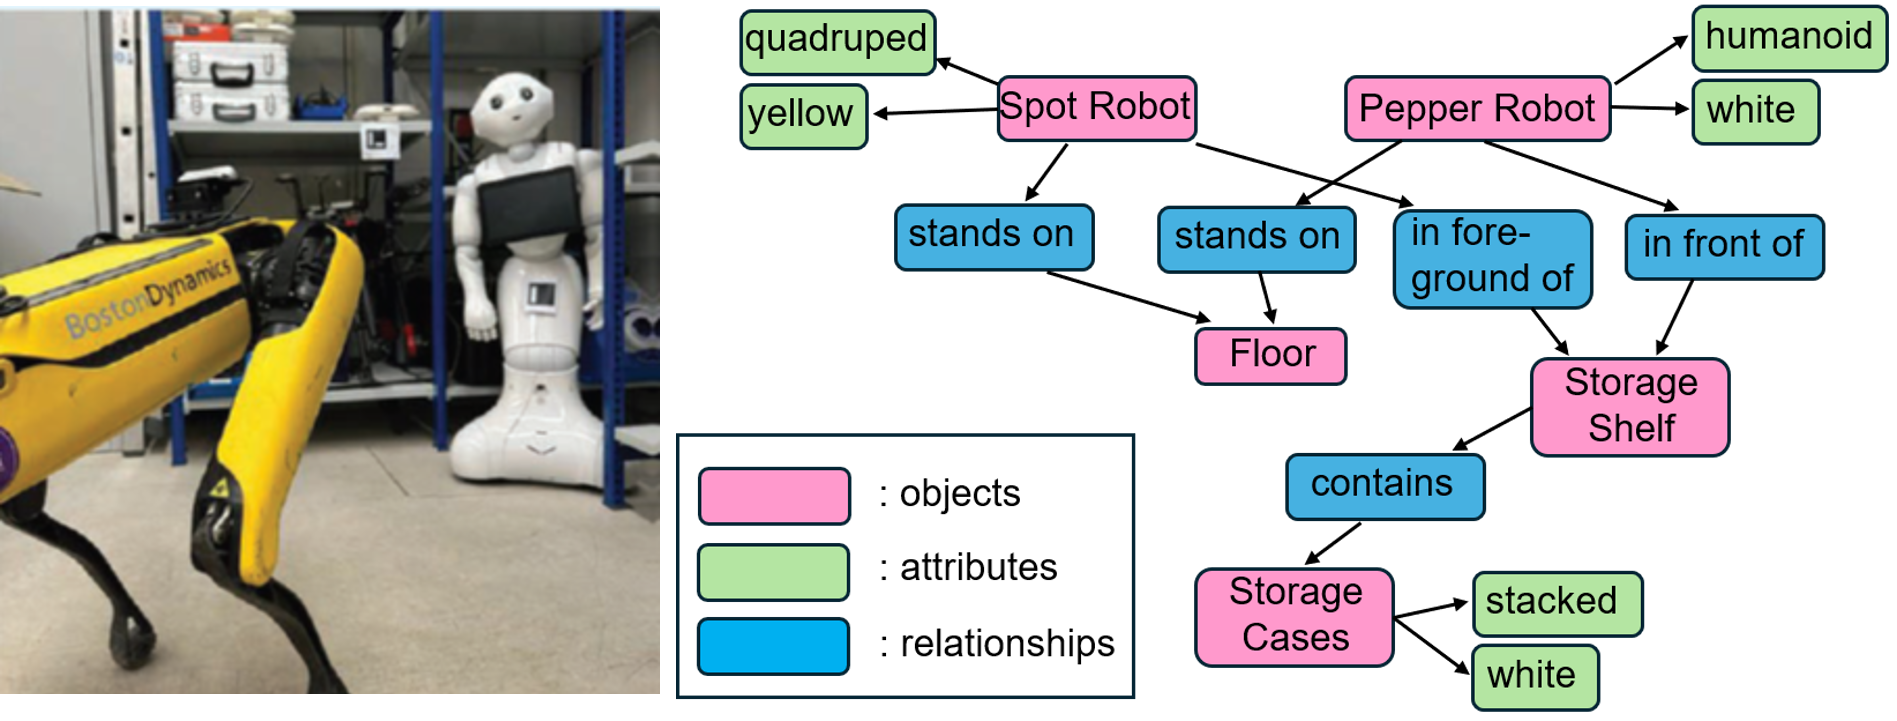
\includegraphics[width=\columnwidth]{Figures/SG_example_small.png}
    \caption{Example image of a scene (left) and related scene graph (right).}
    \label{fig:SG_example}
\end{figure}

The generation of scene graphs is mainly based on machine learning approaches and can be 
roughly divided into three parts: feature extraction, contextualization, and graph construction and reasoning \cite{li2024scene}. Herein, the process of feature extraction is mainly responsible for encoding objects or object pairs in the image. Contextualization plays the role of associating different
entities and is mainly used to enhance the contextual information between entities. Finally, 
this contextual information is used to predict the predicate and complete the construction and inference of the graph. There are currently two main types of scene graph generation \cite{li2024scene}, \cite{chang_comprehensive_2023}. The top-down methods comprise two sequential stages, namely object detection and pairwise relationship recognition, while the bottom-up method involves jointly detecting and recognizing the objects and their relationships \cite{adaimi2023composite}. 

As scene graphs can abstract objects and the relationships between them in a more explicit and easier-to-understand way, they became quite popular for visual scene understanding in general computer vision, but also in robotics. The conceptual shift from dense, low-level metric maps towards scene graphs represents a significant advancement in robotic world modeling. In robotics, scene graphs offer an abstract, layered representation that bridges the gap between the raw geometric perception and high-level symbolic reasoning \cite{bavle_slam_2023}. By decomposing an environment into a scene graph structure robots can move beyond flat representations, such as occupancy grids or point clouds, to models that capture the semantic and relational architecture of the world.  

As scene graphs might rapidly grow in real-world complex environments, the literature distinguishes between two primary structural paradigms: 
\begin{itemize}
    \item Flat Scene Graphs: these models treat all entities equally at a single level of representation, focusing on object-level nodes and their direct relationships \cite{catalano_3d_2025}. Approaches such as ConceptGraphs\cite{gu_conceptgraphs_2023} and SceneGraphFusion\cite{wu_scenegraphfusion_2021} utilize this approach to manage open-vocabulary object recognition and incremental updates in cluttered scenes where clear structural hierarchies may be emergent rather than predefined. 
    \item Hierarchical Scene Graphs: these represent the environment across multiple levels of abstraction, grouping lower level elements into semantically richer containers, e.g. objects within rooms, rooms within buildings\cite{rosinol_3d_2020} \cite{bavle_s-graphs_2025}. This multi-resolution approach is crucial for scalability in large-scale environments, as it allows robots to perform long-term planning and inference over compact abstractions rather than dense data \cite{catalano_3d_2025}.  
\end{itemize}
Hierarchical frameworks like Hydra \cite{hughes_hydra_2022} or S-Graphs\cite{bavle_s-graphs_2025} adopt a bottom-up stack comprising distinct layers specifically for indoor environments: (1) Metric-Semantic Mesh, Pointcloud, (2) Objects and Agents, (3) Places and Structures, (4) Rooms and Floors, and (5) Building. An example that extends these works to outdoor scenes is  \cite{greve_collaborative_2024} that proposes a hierarchical scene graph of a traffic scenario comprising 6 layers: (1) Keyframes \& Point clouds, (2) Lane Graph, (3) Vehicles, (4) Landmarks, (5) Roads \& Intersections, and (6) Environment.

As real-world scenes are three-dimensional, the idea of scene graphs has been extended to 3D space, leading to 3D scene graphs (3DSG) \cite{armeni_3d_2016} \cite{kim_3-d_2020}. 
Edges in a 3DSG encode the connections within the world model through several relationship types, such as: 
\begin{itemize}
    \item Spatial Relations: These include geometric constraints such as \textit{on}, \textit{in}, \textit{adjacent to} and \textit{support} \cite{catalano_3d_2025} \cite{yan_dynamic_2025}.
    \item Visibility and Proximity: \textit{Co-visibility} edges link objects seen simultaneously, while \textit{close-to} edges often use nearest-neighbor  k-d tree to define spatial proximity \cite{behrens_lost_2025}.
    \item Functional Relations: a newer class of edges representing operational dependencies. OpenFunGraph models these as directed edges between ``interactive elements'', such as switches and handles, and objects that they influence, e.g. \textit{controls} a light, \textit{opens} a cabinet \cite{zhang_open-vocabulary_2025}.
    \item Affordances: attributes or edges that define possible interactions which can change the entities' states, such as \textit{sit on}, \textit{opening}, \textit{pulling}, providing the robot with actionable knowledge \cite{catalano_3d_2025}.
    \item Containment and Affiliation: Inter-layer edges such as \textit{part of}, \textit{located in} or \textit{contains} facilitate hierarchical queries \cite{catalano_3d_2025} \cite{behrens_lost_2025}.
\end{itemize}
This structured abstraction allows robots to move beyond simple obstacle avoidance, static mapping and localization, towards actionable spatial perception, where the world model serves as a persistent, queryable memory for complex multi-step tasks in evolving robot-human shared spaces. Two examples of a 3DSG are shown in Figure \ref{fig:Examples_3DSG}.
\begin{figure}[ht]
    \centering
    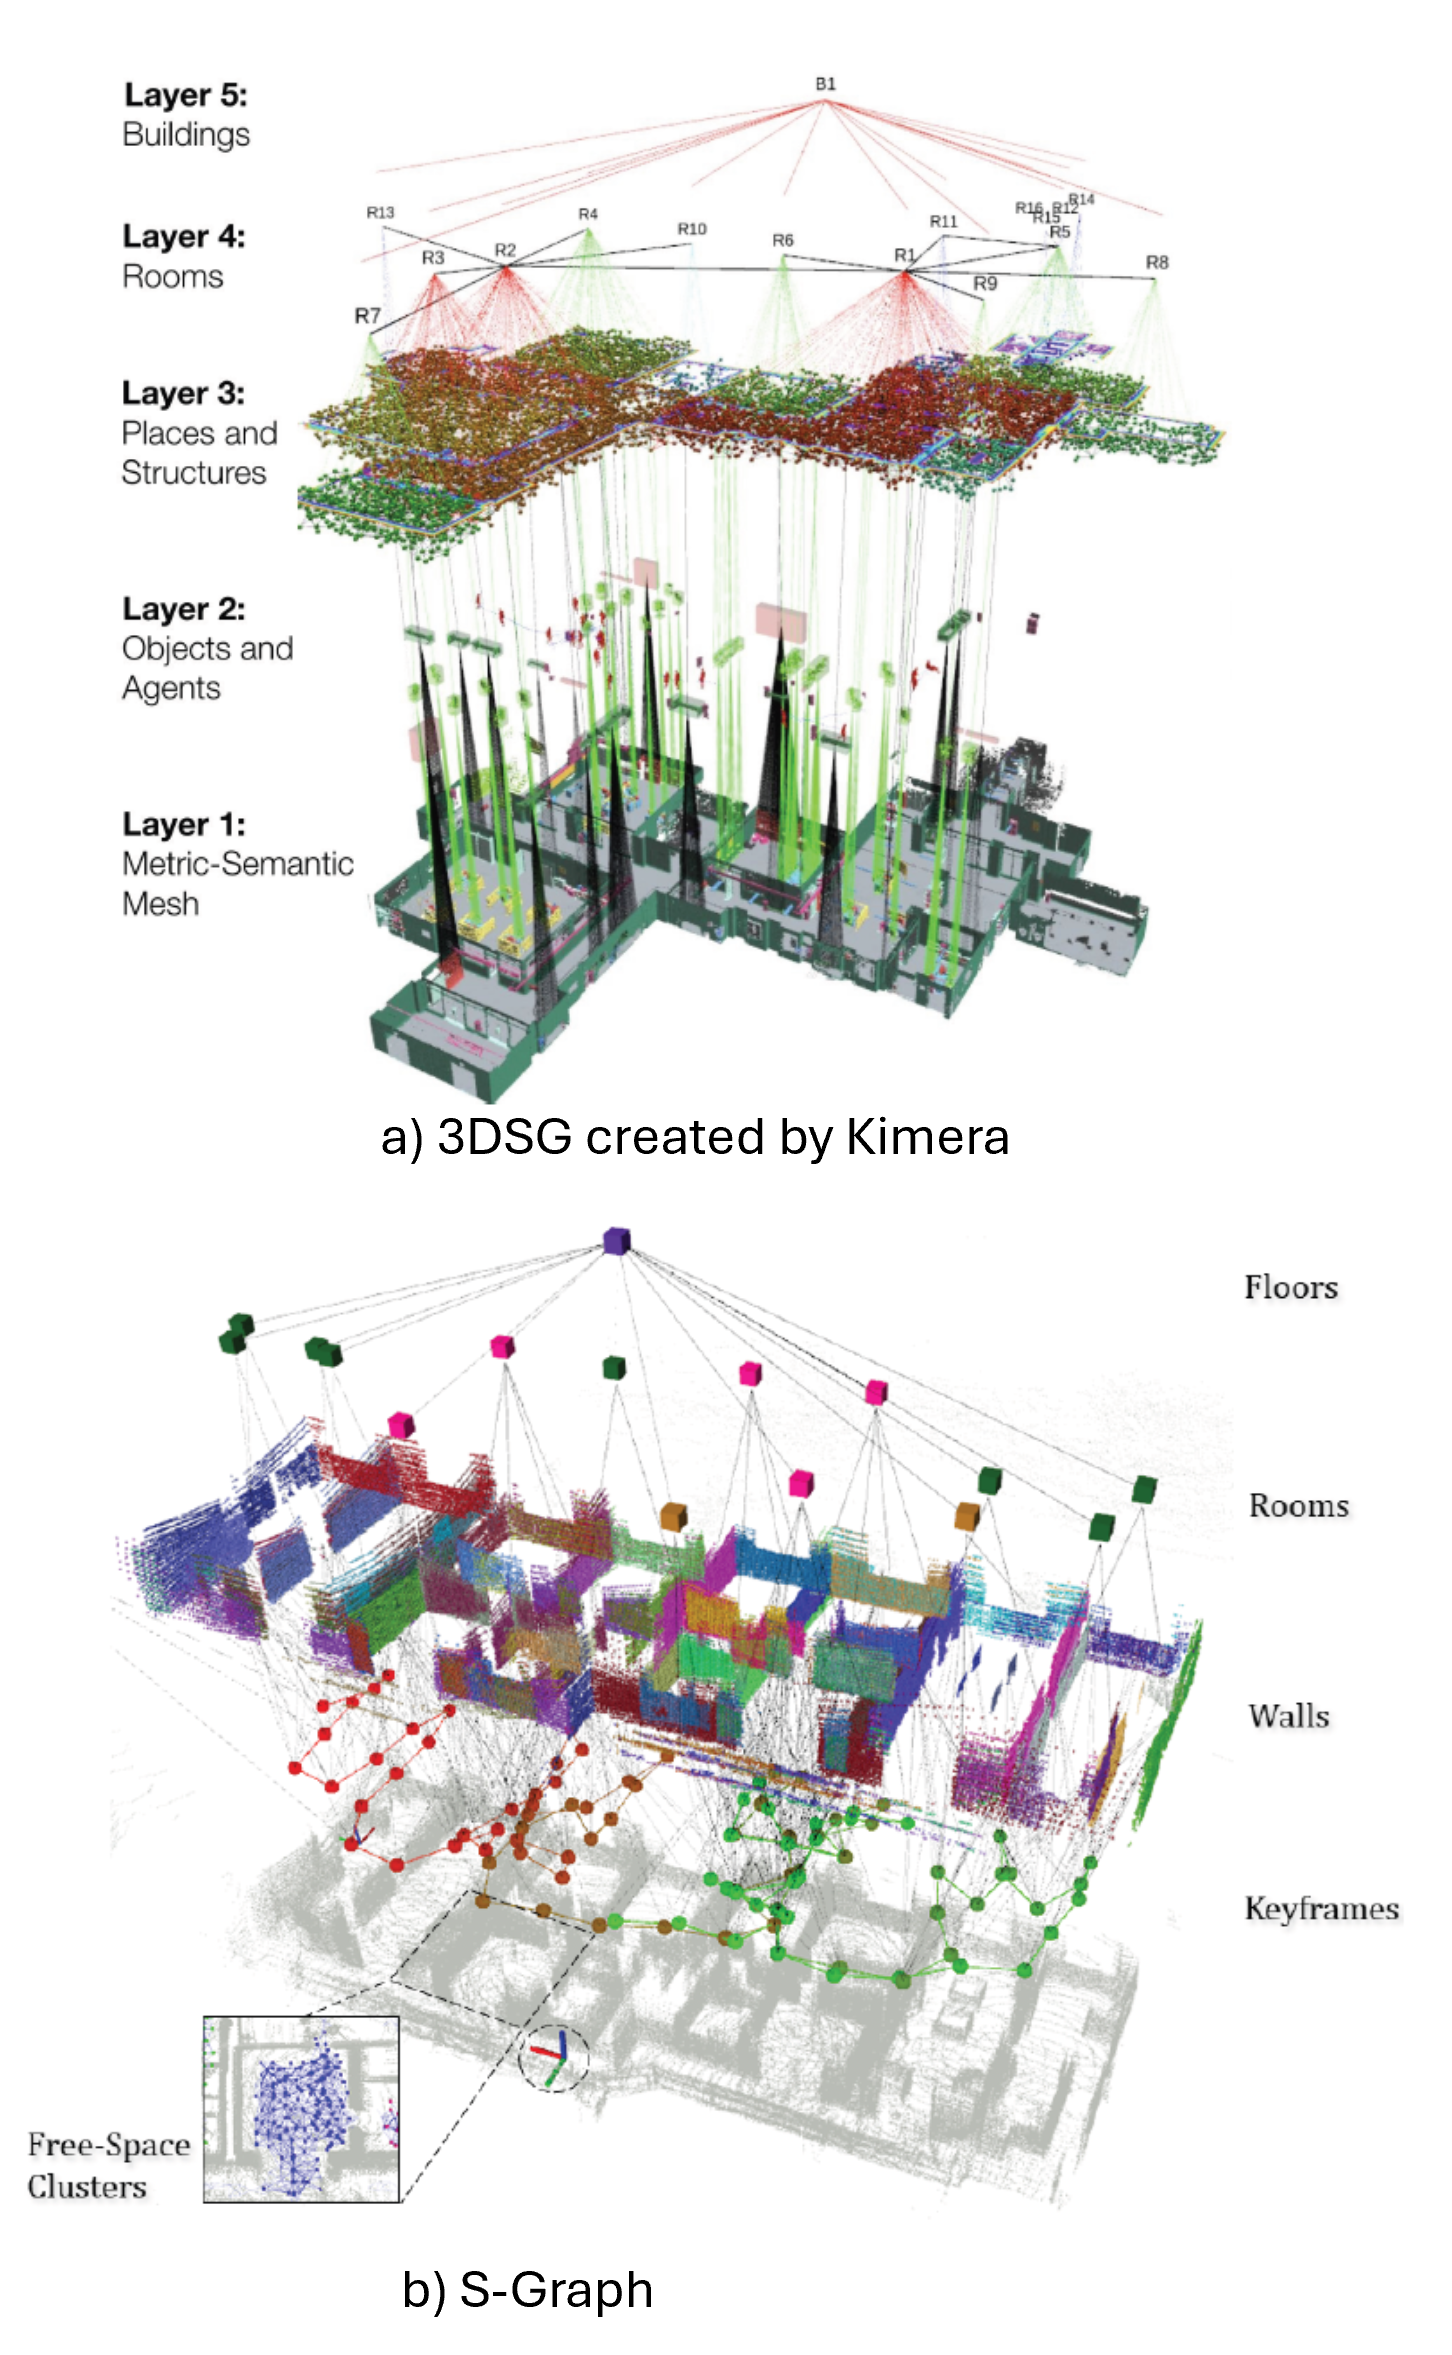
\includegraphics[width=\columnwidth]{Figures/Examples_3DSG.png}
    \caption{Example of 3DSGs created by (a) Kimera \cite{rosinol_kimera_2021} and (b) S-Graphs \cite{bavle_situational_2022}.}
    \label{fig:Examples_3DSG}
\end{figure}

\subsubsection{Hybrid Models using Factor and Scene Graphs}\label{sec:background_hybrid}
A scene graph answers \textit{``what exists and how it relates''}, while a factor graph answers \textit{``where it is, and how certain, consistent it is with sensor measurements''}.
This complementarity motivates hybrid architectures that combine the two paradigms within a common world representation, without implying that such architectures are generally superior to either paradigm in isolation.
Recent robotics 3DSG solutions explicitly include a pose-graph layer as the uncertainty-bearing backbone, and the integration of the two paradigms creates a multi-resolution framework which bridges metric-semantic perception with high-level symbolic reasoning \cite{rosinol_kimera_2021} \cite{bavle_situational_2022}.
In this hybrid paradigm, factor graphs serve as the probabilistic geometric backbone, while scene graphs provide the relational architecture necessary for task-level autonomy in dynamic environments \cite{catalano_3d_2025} \cite{rosinol_3d_2020}.

In this review, we use the term hybrid factor graph-scene graph (FG-SG) architecture in an operational sense. 
A system is considered hybrid when it explicitly maintains both a factor-graph-based estimation structure and a scene-graph representation of semantic entities and their relations, with explicit cross-representation correspondences between states or entities represented in the two structures.
This distinguishes hybrid FG-SG architectures from conventional semantic SLAM systems, in which semantic labels, object landmarks, or semantic priors may be incorporated into the SLAM graph without constructing a separate relational scene-graph representation.
Bidirectional information flow is not required for a system to be considered hybrid. Instead, the direction of information flow and, crucially, whether the two representations participate in a common optimization objective determine the form and degree of coupling.

% \hl{In this review, we use the term factor graph-scene graph (FG-SG) hybrid in an operational sense. 
% A system is considered hybrid when it explicitly maintains both a factor-graph-based estimation structure and a scene-graph representation of semantic entities and their relations, with an explicit correspondence or information exchange between the two.
% This distinguishes FG-SG hybrids from conventional semantic SLAM systems, in which semantic labels, object landmarks, or semantic priors may be incorporated into the SLAM graph without constructing a separate relational scene-graph representation.
% The existence of bidirectional feedback is therefore not required for a system to be considered hybrid, rather, the direction and magnitude of this information exchange determine its degree of coupling.} 

The literature converges to a small set of recurring architectural patterns for coupling the two paradigms, distinguished primarily by information-flow direction and optimization ownership. 
We first distinguish loosely coupled architectures, in which the factor graph and scene graph remain outside a common optimization objective, from tightly coupled architectures, in which scene-graph-level entities or constraints participate directly in the estimation graph. 
Within the loosely coupled class, we further distinguish layered/feed-forward and parallel architectures according to whether the scene graph is constructed downstream from the factor-graph output or maintained as a separate representation.

The first loosely coupled pattern is the \textbf{layered, feed-forward} \textbf{stack with factor graph backbone}: the factor graph simultaneously optimizes the robot's trajectory and the metric-semantic mesh, whose globally and temporally consistent output is then fed to a separate scene graph parser that builds the relational structure on top. 
Hydra \cite{hughes_hydra_2022} and Kimera \cite{rosinol_kimera_2021} support this approach, where a dedicated parsing thread incrementally constructs the scene graph from the optimized metric layer. 
The advantage is modularity, where the scene graph logic can be developed independently of the SLAM back-end, but the disadvantage is a one-directional information flow: the scene graph is informed by the factor graph, but semantic information rarely propagates back to improve localization.

The second loosely coupled pattern is the  \textbf{parallel architecture}, in which  the factor graph and scene graph are maintained as separate representations   and synchronize corresponding entity states or node positions through explicit cross-representation correspondences. Unlike the layered feed-forward case, the scene graph is maintained as a persistent representation rather than being constructed solely as a downstream product of the factor-graph output. Unlike the unified case, however, scene-graph-level states and constraints do not participate in the factor graph's optimization objective. This preserves modularity and reduces optimization complexity at the expense of weaker consistency guarantees \cite{rosinol_3d_2020}.

The tightly coupled pattern is the \textbf{unified optimizable graph}, in which scene graph entities are incorporated directly as variables and factors within the same factor graph that optimizes robot poses. 
S-Graphs \cite{bavle_s-graphs_2025} and its visual counterpart vS-Graphs \cite{tourani2026vs} introduced this pattern, merging SLAM and scene graph into a single multi-layered jointly optimizable factor graph where walls, rooms, and floors appear as semantic variables constrained by geometric factors.
This enables bidirectional information flow: geometric observations constrain semantic entity positions, but semantic structural priors in turn constrain and regularize ego-trajectory estimation, demonstrably reducing drift compared to purely geometric approaches.
The defining distinction from loosely coupled architectures is therefore participation of scene-graph-level states or constraints in the common estimation objective, rather than bidirectional information exchange alone.
\hl{The degree of architectural coupling should also be distinguished from the extent of uncertainty propagation.
A loosely coupled architecture can explicitly transfer uncertainty estimates between its constituent representations without performing joint optimization. Conversely, joint optimization does not necessarily imply that all uncertainty classes are explicitly modeled or that their posterior uncertainties are computed and made available to other representation layers.}

\subsection{Dynamics in the Context of Robotics}\label{sec:background_dynamics_definition}
It is necessary to fix what we mean by \textit{dynamics}, since the term is used inconsistently across robotics and adjacent fields. 
In classical mechanics, dynamics concerns forces and torques and their effect on motion; in dynamical system theory, it describes the time-evolution of a point in a geometric state space; in computer science, a ``dynamic'' data structure refers to memory organization rather than physical change. 
Within mobile robotics, the term is used more narrowly and typically refers to external, uncontrolled moving entities, such as pedestrians and vehicles, that a robot must perceive and account for during localization and mapping\cite{kucner_survey_2023}. 

This robotics-specific usage, however, is itself too narrow for our purpose.
Hahnel et al. \cite{hahnel2003map} offered one of the first attempts to define dynamics as an environmental property, stating that an environment is dynamic if it changes over time or if moving objects are present within it. 
This definition is useful but indirect, and, being framed around discrete macroscopic objects, does not make explicit how motion that is never directly observed, e.g. a chair found in a new location, should be treated. Therefore, we adopt the definition of dynamics given in \cite{kucner_survey_2023}:
\vspace{6pt}
\begin{definition}[Dynamics]
\label{def:dynamics}
    Dynamics are any directly or indirectly perceivable motions.
\end{definition}
\vspace{6pt}
This formulation is deliberately broad. \textit{Direct} perceivability covers motion observed as it occurs given an appropriate sensor.
\textit{Indirect} perceivability covers semi-static entities, such as relocated furniture, whose motion is never itself observed but whose resulting change of state is.
This distinction between direct and indirect perceivability, rather than any specific list of entity types or timescales, is what we take to be the essential content of Definition \ref{def:dynamics}, and it is this distinction, not a fixed taxonomy, that Kucner et al. \cite{kucner_survey_2023} leave open for further specialization within a given application domain.

Definition \ref{def:dynamics} tells us \textit{what} qualifies as dynamics. It does not by itself prescribe how a world model should organize or respond to different instances of it.
In Section \ref{sec:taxonomy_dynamics}, we build on this definition to introduce a taxonomy of dynamics tailored to graph-based robotic world models, organized primarily around the temporal horizon at which a perceivable motion or change occurs.

\begin{comment}
 
In the previous sections, we relied on an intuitive under-
standing of such fundamental terms as dynamics or maps.
However, both terms are widely used across different fields,
and their definitions vary from field to field. For instance, in
the field of classical mechanics, dynamics concern the study
of forces and torques and their effect on motion. A dy-
namical system in mathematics refers to a system in which a
function describes the time dependence of a point in a
geometrical space. In computer science, a dynamic data
structure refers to an organization or collection of data in
memory that has the flexibility to grow or shrink in size.
In the context of mobile robotics the term dynamics is
much less ambiguous and is usually used to describe ex-
ternal, uncontrolled moving entities. That said, this term is
not often used in relation to environmental features. Thus, to
apply this term in the context of MoDs, there is a need to
redefine it. The first attempt to define dynamics as an en-
vironmental feature was proposed by H¨ahnel et al. (2003).
In their work, the authors state that an environment is
dynamic if it changes or if moving objects are present
therein. This indirect definition of dynamics is formulated
such that it primarily focuses on macroscopic objects.
Meanwhile, contemporary robotics finds its application in a
multitude of environments where not only macroscopicdiscrete objects are dynamic. In fields like aerial and marine
robotics, the dynamics also include the flow of water and air,
respectively. Thus, the definition by H¨ahnel et al. (2003)
does not cover such types. To mitigate this limitation, we
propose the following definition of dynamics in the context
of robotics:
\begin{definition}[Dynamics]
\label{def:dynamics}
Dynamics are any directly or indirectly perceivable motions.
\end{definition}
Such a formulation of dynamics captures both motion of
discrete objects and continuous media (they are both per-
ceivable with adequate sensors, that is, anemometers,
speedometers, radars)
This definition further includes semi-static objects. For
such objects (i.e. chairs, cars), the motion is not per-
ceivable directly (the motion of an actual object has not
been perceived), but the result (indirect observation) can
be.
\end{comment}

\subsection{Assessment of Previous Surveys and Reviews}
% FG
Probabilistic Graphical Models provide the foundational framework for modeling large-scale inference problems in robotics, with factor graphs serving as a bipartite representation where variables denote unknown states and factors represent local constraints derived from sensor data \cite{dellaert_factor_2021} \cite{dellaert_factor_2017}.
Traditional reviews trace the maturity of SLAM from early formulations based on Kalman filters and Bayesian estimation toward modern graph-based optimization paradigms \cite{mascaro_scene_2025} \cite{luca_carlone_slam_2025}.
Systematic surveys of spatial perception frameworks have categorized scene modeling techniques into three primary layers: metric, metric-semantic, and metric-semantic-topological \cite{mascaro_scene_2025}. 
This highlights a trend shifting away from purely geometric representations like point clouds or meshes, toward advanced data structures that incorporate high-level concepts such as instances and places \cite{bavle_slam_2023}.

% SG
Complementary to reviews of metric frameworks, existing reviews of scene graphs define them as structured representations that encode semantic entities and their interrelationships to facilitate human-like reasoning \cite{chang_comprehensive_2023} \cite{amuche_advancements_2025} \cite{lai_review_2022}. 
Early literature in this domain primarily focused on offline image retrieval and 2D scene graph generation, though more recent reviews highlight advancements in 3D scene graphs capable of capturing metrics, semantics and objects (also including dynamic agents) within a unified actionable model \cite{chang_comprehensive_2023} \cite{lai_review_2022}.

Notably, these two types of reviews have developed largely independently: reviews of factor graphs assess uncertainty-aware geometric estimation, while reviews of scene graphs assess semantic and relational abstraction, but very few works survey both representations \emph{jointly} as complementary layers of a single world model. A first recent attempt in this direction is the review of Catalano et al. \cite{catalano_3d_2025}, which focuses on works that combine geometry, semantics, and action within unified representations; however, this overview  does not center on dynamics, nor does it systematically analyze the coupling patterns, uncertainty propagation, or construction pipelines that arise when factor and scene graphs are combined specifically to handle non-stationary environments.

% Dynamic SLAM
The landscape of SLAM in dynamic environments has been analyzed as a progressive evolution from purely geometric methods to advanced semantic-based paradigms \cite{wang_survey_2024} \cite{chen_semantic_2025} \cite{wen_semantic_2021}.
Existing surveys categorize solution approaches into those that maintain localization stability by excluding dynamic elements as outliers and those that perform active Simultaneous Localization, Mapping and Moving Object Tracking (SLAMMOT) \cite{wang_-depth_2025} \cite{xu_survey_2021}. 
Furthermore, dedicated reviews on feature requirements in dynamic SLAM weight the trade-offs between low-level primitives, such as points or lines, and high-level semantic labels, suggesting that robust robotic autonomy may require the integrated usage of both feature levels \cite{xu_survey_2021}.
These dynamic-SLAM surveys, however, largely set aside the scene-graph literature, and consequently do not address how semantic-relational structure should be maintained under dynamics, nor how it interacts with the probabilistic backbone of the factor graph.

A separate line of work addresses dynamics as a phenomenon in its own right, independent of any specific representation. Kucner et al.\cite{kucner_survey_2023} survey Maps of Dynamics (MoDs) and propose a general definition and characterization of dynamics for mobile robotics, which we adopt and extend in Section \ref{sec:background_dynamics_definition} and organize into a temporal-horizon taxonomy in Section~\ref{sec:taxonomy_dynamics}. 
While their survey provides a rigorous treatment of \textit{what} dynamic phenomena are and how they can be statistically modeled over space and time, it is agnostic to the underlying world-model representation, and does not address factor graphs, scene graphs, or their hybrid forms.

% Identified gaps
Despite the depth of reviews in individual subfields, critical gaps in the existing review or survey literature can be identified.  
Key surveys often focus on isolated areas like perception or planning while overlooking the practical integration of these components \cite{khan_foundation_2025} \cite{bavle_slam_2023}.
Gaps also remain in analyzing the long-term usability of maps in complex dynamic scenes and handling the non-rigid deformations inherent in highly dynamic environments \cite{chen_semantic_2025} \cite{luca_carlone_slam_2025}.
Taken together, these limitations reveal a fragmented landscape in which probabilistic estimation (factor graphs), semantic scene understanding (scene graphs), and the characterization of dynamics have each matured in relative isolation, with limited cross-pollination between the three. 
To the best of our knowledge, no existing survey or review jointly addresses the full pipeline from probabilistic spatio-temporal estimation to structured semantic reasoning especially in \textit{dynamic} environments, nor does any work systematically analyze how these two paradigms can be combined to achieve robust, long-term or even lifelong situational awareness.

This review addresses these gaps directly.
We first establish a shared characterization of dynamics (Section~\ref{sec:taxonomy_dynamics}), building on and extending the definition of Kucner et al. \cite{kucner_survey_2023} and based on the surveyed literature, and then assess existing works with respect to three questions: which graph-based representations are suited to dynamic environments (Section ~\ref{sec:dyn_world_model_representations}), how they are constructed and maintained (Section ~\ref{sec:construction_pipeline}), and how they are exploited for downstream tasks (Sections~\ref{sec:querying_reasoning_action}--\ref{sec:applications}). 
Additionally, we present the commonly used evaluation protocols, datasets, and metrics for testing in ~\ref{sec:evaluation_metrics}, and a  structured comparison of  representative related works in ~\ref{sec:taxonomy}. Finally, we conclude this review by highlighting the open challenges identified and outlining future research directions in ~\ref{sec:challenges_future_works}. 
In doing so, this review provides a unified perspective on the synergy between factor graphs and scene graphs as complementary and mutually reinforcing tools for long-term robotic autonomy under dynamics.


\subsection{Review Scope and Literature Selection}
The literature corpus was assembled through targeted searches of IEEE Xplore, Google Scholar, and arXiv, complemented by backward and forward citation tracing from key surveys and representative works.
The primary search covered publications from 2012 to July 2026, while earlier works were retained where needed to establish methodological foundations.
Search concepts combined terms related to \textit{factor graphs}, \textit{scene graphs}, \textit{dynamic SLAM}, \textit{dynamic world models}, \textit{spatio-temporal mapping}, \textit{lifelong mapping}, \textit{multi-object tracking}, and \textit{semantic/relational mapping}.
% We included robotic systems that employ factor graphs, scene graphs, or their combination to represent, construct, maintain or exploit world models under environmental dynamics.
% Static-only mapping, perception-only methods without a persistent world representation, and works outside robotics were excluded unless directly relevant to the emerging trends discussed in this review. 
% The systems in Table} \ref{tab:taxonomy_overview} \hl{were selected as representative examples spanning the main graph-stack architectures, dynamic regimes, inference strategies, uncertainty treatments, and downstream uses identified in the survey.
% As a topical rather than systematic review, the resulting corpus is intended to be broad and representative rather than exhaustive, particularly for the rapidly evolving preprints and adjacent emerging representations.
Candidate works were included when they: (i) addressed a robotic mapping, world-modeling, tracking or scene-understanding problem; (ii) employed factor graphs, scene graphs, or their combination as a substantive component of the maintained representation or inference architecture; and (iii) addressed environmental dynamics or contributed directly to one of the representation, construction/maintenance, or exploitation questions considered in this review.
Earlier static or methodological works were retained when required to establish the foundations of techniques subsequently used for dynamic world modeling.
Static-only mapping systems, perception-only methods without a persistent world representation, and works outside robotics were excluded unless directly required for methodological context.
The comparative systems in Table \ref{tab:taxonomy_overview} constitute a representative rather than exhaustive subset of this corpus. 
Systems were selected when they instantiated one of the main FG, SG, or hybrid architectural patterns identified in the review, treated environmental dynamics as a substantive part of the method, and provided sufficient information to characterize the comparison axes introduced in Section \ref{sec:taxonomy}. Where several closely related works instantiated the same architecture, preference was given to the most complete or representative system description, while other works were retained when they introduced a distinct formulation or capability.

The review adopts a structured topical-review methodology designed to provide broad coverage of the principal graph-based approaches to dynamic robotic world modeling.
The combination of database searches, citation tracing and explicit selection criteria was used to capture the main methodological developments, architectural patterns, and representative systems relevant to the scope of the review.
Given the breadth and rapid evolution of the field, the identified trends and research gaps should be interpreted within the scope and selection criteria defined above.
